\documentclass[class={IEEEtran}]{standalone}

\usepackage{amsmath}
\usepackage{tikz}
\usepackage{pifont}

\newcommand{\whiteding}[1]{\large{\ding{\numexpr171+#1\relax}}}

\pagestyle{empty}

\usetikzlibrary{shapes.geometric,shapes.arrows,positioning,calc,arrows.meta,math}

\tikzset{AGENT/.style={rectangle,minimum width=6.5em,minimum height=3.5ex,draw,semithick,align=flush center, anchor=north}}
\tikzset{ACTION/.style={rectangle,rounded corners,draw,semithick,align=flush center,fill=white}, anchor=north}
\tikzset{ARROW/.style={thick, -stealth}}
\tikzset{DARROW/.style={<->,>=latex, line width=4ex, gray!20}}
\tikzset{PREPARATION/.style={rectangle,draw,semithick,align=flush center,fill=white,dashed, anchor=north}}


\begin{document}
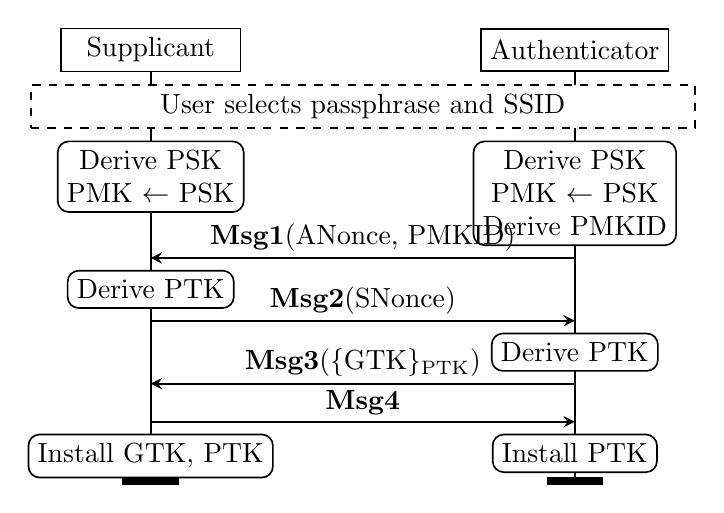
\begin{tikzpicture}

\node[AGENT] (n_station) {Supplicant};
\node[AGENT, right=0.25\textwidth of n_station] (n_ap) {Authenticator};

\coordinate (end_station) at ($(n_station.south)+(0,-34ex)$);
\draw[semithick] (n_station.south) -- (end_station);
\draw[fill=black] ($(end_station)+(-1em,0)$) rectangle ($(end_station)+(1em,-0.6ex)$);

\coordinate (end_ap) at ($(end_station-|n_ap)$);
\draw[semithick] (n_ap.south) -- (end_ap);
\draw[fill=black] ($(end_ap)+(-1em,0)$) rectangle ($(end_ap)+(1em,-0.6ex)$);

\coordinate (c_middle) at ($(n_station.south)!0.5!(n_ap.south)$);
\node[PREPARATION, minimum width=24em] (n_prep) at ($(c_middle)+(0, -1ex)$) {User selects passphrase and SSID};

\node[ACTION] (n_station_pmk) at ($(n_prep.south-|n_station)+(0,-1ex)$) {Derive PSK \\ PMK $\leftarrow$ PSK};
\node[ACTION] (n_ap_pmk) at ($(n_prep.south-|n_ap)+(0,-1ex)$) {Derive PSK \\ PMK $\leftarrow$ PSK \\ Derive PMKID};

\coordinate (c_msg1_ap) at ($(n_ap_pmk.south)+(0,-1ex)$);
\coordinate (c_msg1_st) at ($(c_msg1_ap-|n_station)$);
\draw[ARROW] (c_msg1_ap) -- (c_msg1_st) node[midway,above=-0.3ex]{\textbf{Msg1}(ANonce, PMKID)};

\node[ACTION] (n_station_anonce) at ($(c_msg1_st)+(0,-1ex)$) {Derive PTK};

\coordinate (c_msg2_st) at ($(n_station_anonce.south)+(0,-1ex)$);
\coordinate (c_msg2_ap) at ($(c_msg2_st-|n_ap)$);
\draw[ARROW] (c_msg2_st) -- (c_msg2_ap) node[midway,above=-0.3ex]{\textbf{Msg2}(SNonce)};

\node[ACTION] (n_ap_snonce) at ($(c_msg2_ap)+(0,-1ex)$) {Derive PTK};

\coordinate (c_msg3_ap) at ($(n_ap_snonce.south)+(0,-1ex)$);
\coordinate (c_msg3_st) at ($(c_msg3_ap-|n_station)$);
\draw[ARROW] (c_msg3_ap) -- (c_msg3_st) node[midway,above=-0.3ex]{\textbf{Msg3}($\{\text{GTK}\}_\text{PTK}$)};

\coordinate (c_msg4_st) at ($(c_msg3_st)+(0,-3.2ex)$);
\coordinate (c_msg4_ap) at ($(c_msg4_st-|n_ap)$);
\draw[ARROW] (c_msg4_st) -- (c_msg4_ap) node[midway,above=-0.3ex]{\textbf{Msg4}};

\node[ACTION] (n_station_gtk) at ($(c_msg4_st)+(0,-1ex)$) {Install GTK, PTK};
\node[ACTION] (n_ap_gtk) at ($(c_msg4_ap)+(0,-1ex)$) {Install PTK};


\end{tikzpicture}




\end{document}
